\documentclass[usenames,dvipsnames]{beamer}
%\documentclass[usenames,dvipsnames,handout]{beamer}


\usetheme{AnnArbor}
% \usecolortheme{default}
% \usecolortheme{crane}
\usecolortheme{beaver}
\usecolortheme{dolphin}
% \usecolortheme{orchid}
% \usecolortheme{rose}


\usepackage{fourier}
\usepackage{faktor}
\usepackage{amssymb}
\usepackage{amsmath}
\usepackage{amsthm}
\usepackage{stmaryrd}
\usepackage{hyperref}
\usepackage[all]{xy}
\newcommand{\downmapsto}{\rotatebox[origin=c]{-90}{$\large\mapsto$}\mkern2mu} %MnSymbol doesn't work well with beamer

\def\Q{\mathbb{Q}}
\def\Z{\mathbb{Z}}
\def\C{\mathbb{C}}
\def\R{\mathbb{R}}
\def\F{\mathbb{F}}

\DeclareMathOperator{\AV}{AV}
\DeclareMathOperator{\Mat}{Mat}
\DeclareMathOperator{\Pol}{Pol}
\DeclareMathOperator{\Char}{char}
\DeclareMathOperator{\rk}{Rank}
\DeclareMathOperator{\Frob}{Frob}
\DeclareMathOperator{\ICM}{ICM}
\DeclareMathOperator{\Pic}{Pic}
\DeclareMathOperator{\Aut}{Aut}
\DeclareMathOperator{\End}{End}
\DeclareMathOperator{\mSpec}{mSpec}

\newcommand{\cC}{{\mathcal C}}
\newcommand{\cO}{{\mathcal O}}
\newcommand{\cW}{{\mathcal W}}

\newcommand{\p}{{\mathfrak p}}
\newcommand{\frf}{{\mathfrak f}}

\newcommand{\set}[1]{\left\lbrace#1\right\rbrace }

\newcommand{\AVord}[1]{\AV^{\text{ord}}({#1})}
\newcommand{\Modord}[1]{\cM^{\text{ord}}({#1})}

\newcommand{\red}[1]{\textcolor{red}{#1}}
\newcommand{\blue}[1]{\textcolor{blue}{#1}}
\newcommand{\green}[1]{\textcolor{ForestGreen}{#1}}

\newtheorem{df}{Definition}[section]
\newtheorem{remark}[df]{Remark}

%AUTHOR DETAILS
%%%%%%%%%%%%%%%%%%%%%%%%%%%%%%%%%%%%%%%%%%%%%%%%
\title[]{Isomorphism classes of abelian varieties over finite fields}
\subtitle{}
\author[Marseglia Stefano]{Marseglia Stefano}
\institute[]{Utrecht University}
\date[28 November 2019]{DIAMANT symposium - 28 November 2019}

\begin{document}

\begin{frame}
\titlepage
\end{frame}

\begin{frame}{ Introduction: Abelian Varieties }
\begin{itemize}
 \item An \green{abelian variety} over a field $k$ is a projective connected group variety over $k$.
 \pause \item e.g. AVs of dim $1$ are elliptic curves:
 \[\text{when }\Char(k)\neq 2,3 \leadsto Y^2=X^3+AX+B  \]
 \vspace{-2em}\pause \item \red{Goal}: compute \textbf{isomorphism classes} of abelian varieties over a \textbf{finite field} (+ extra structure, like polarizations, period matrices, etc.)
 \pause \item in dimension $g>1$ is not easy to produce equations.
% \pause \item for $g>3$ it is not enough to consider Jacobians.
 \pause \item over $\C$:
 \[
      \set{ \text{abelian varieties $/\C$} } \longleftrightarrow 
      \set{\parbox[c]{10em}{$\C^g/L$ with $L\simeq \Z^{2g}$ with\\eq.cl.~of Riemann form}}
 \]
 \pause \vspace{-6mm} \item in positive characteristic we don't have such equivalence.
\end{itemize}
\end{frame}

\begin{frame}{ Classification problem }
	\begin{itemize}
		\item $A$ and $B$ are \green{isogenous} if $\dim A=\dim B$ and there exists a surjective homomorphism $\varphi:A\to B$.
		\pause \item Being isogenous is an equivalence relation.
		\pause \item $A/\F_{p^r}$ comes with a \blue{Frobenius endomorphism}, that induces an action
		\[ \Frob_A : T_\ell A \rightarrow T_\ell A \text{ for any }\ell\neq p. \]
		$\Char(\Frob_A)$ is a \blue{$p^r$-Weil polynomial}.
		\pause \item By \red{Honda-Tate} theory, the association
		\[ \text{isogeny class of }A \mapsto \Char(\Frob_A)\]
		is injective and allows us to \red{enumerate} all AVs up to isogeny.
	\end{itemize}
\end{frame}

\begin{frame}{ Deligne's equivalence }
\begin{theorem}[Deligne '69]
Let $q=p^r$, with $p$ a prime.
There is an \red{equivalence of categories}:
\[ \begin{array}{cc}
\set{\text{ {\bf Ordinary} abelian varieties over } \F_q } 	& A \\
\pause \updownarrow											& \downmapsto \\
\set{\parbox[p]{19em}{pairs $(T,F)$, where $T\simeq_\Z \Z^{2g}$ and $T\overset{F}{\to} T$ s.t.\\
- $F\otimes \Q$ is semisimple\\
- the roots of $\Char_{F\otimes\Q}(x)$ have abs. value $\sqrt{q}$\\
- \textbf{half of them are $p$-adic units}\\
- $\exists V:T\to T$ such that $FV=VF=q$
}}	& (T(A),F(A))
\end{array} \]

\end{theorem}
\pause
\begin{remark}
\begin{itemize}
 \item If $\dim(A)=g$ then $\rk(T(A))=2g$;
 \item $\Frob(A)\rightsquigarrow F(A)$.
\end{itemize}
\end{remark}
\end{frame}

\begin{frame}{Main result}
	\begin{itemize}
		\item Fix an \textbf{ordinary squarefree} $q$-Weil polynomial \red{$h$} :
\pause  \item  $\rightsquigarrow \text{an isogeny class } \red{\cC_h}$.
\pause 	\item Put $K := \Q[x]/(h)=\Q[F]$.

\pause 	\item Deligne's equivalence induces:
% \vspace{-2 em}
			\begin{theorem}[M.]
			\[\begin{array}{cc}
			\faktor{\set{\text{abelian varieties over $\F_q$ in $\cC_h$}}}{\simeq} & \\
			\updownarrow & \\
			\faktor{\set{ \text{fractional ideals of $\Z[F,q/F] \subset K$ } }}{\simeq} &\pause =:  \green{\ICM(\Z[F,q/F])}\\ 
			& \green{\text{ ideal class monoid} }
			  \end{array}\]
			\end{theorem}
\pause \item \red{Problem: } $\Z[F,q/F]$ might not be maximal $\rightsquigarrow $ \red{non-invertible} ideals.
	\end{itemize}
\end{frame}

\begin{frame}{ICM : Ideal Class Monoid}
Let $R$ be an \green{order} in a finite \'etale  $\Q$-algebra $K$.
% according to Bourbaki etale (over a field K) implies commutative and finite (since it is defined as being isomorphic to L^n for some extension L of K).
\begin{itemize}
   \pause \item Recall: for fractional $R$-ideals $I$ and $J$
	\[ I\simeq_R J \Longleftrightarrow \exists x \in K^\times \text{ s.t.~} xI=J \]
   \pause \item We have
   				\begin{align*}
   					\ICM(R) 	  & \supseteq \Pic(R)=\faktor{\set{\text{invertible fractional $R$-ideals}}}{\simeq_R} \\
	\blue{\text{with equality }} & \blue{\rotatebox[origin=c]{90}{$\large\rightsquigarrow$}\mkern2mu \text{ iff } R=\cO_K }
   				\end{align*}
   \pause \item ...and actually
   \[ \ICM(R) \supseteq \bigsqcup_{\scriptsize\parbox{5 em}{$R\subseteq S \subseteq \cO_K$\\over-orders}}\Pic(S) \qquad \textcolor{blue}{\text{with equality iff $R$ is Bass}} \] 
\end{itemize}
\end{frame}

\begin{frame}{ simplify the problem  }
Study the isomorphism problem locally: (Dade, Taussky, Zassenhaus '62)
\begin{itemize}
\pause \item  \textbf{weak equivalence}:
	\[I_{\p}\simeq_{R_{\p}} J_{\p} \text{ for every } {\p} \in \mSpec(R)\]
\pause \vspace{-6mm}\[\Updownarrow\]
	\[1\in (I:J)(J:I)\quad \textcolor{blue}{\text{easy to check!}}\]
\pause \item Let $\cW(R)$ be the set of weak eq.~classes...\\
\pause ...whose representatives can be found in
	\[\set{\text{sub-$R$-modules of $\faktor{\cO_K}{\frf_R}$ }} \quad \textcolor{blue}{\parbox{10 em}{finite! and most of the time not-too-big ...}}\]
\end{itemize}
\end{frame}

\begin{frame}{ Compute $\ICM(R)$ }
\pause Partition w.r.t. the multiplicator ring:
    \begin{columns}
    \begin{column}{0.5\textwidth}
      \[ \cW(R) = \bigsqcup_{R\subseteq S \subseteq \cO_K} \cW_S(R)\]
      \[ \ICM(R) = \bigsqcup_{R\subseteq S \subseteq \cO_K} \ICM_S(R)\]
    \end{column}
\pause
    \begin{column}{0.5\textwidth}  %%<--- here
	\begin{center}
	\textcolor{blue}{\parbox{10em}{the ``pedix'' $-_S$ means ``only classes with multiplicator ring S''}} 
	\end{center}
    \end{column}
    \end{columns}
\pause
   \begin{theorem}[M.]
    For every over-order $S$ of $R$, $\Pic(S)$ acts \red{freely} on $\ICM_S(R)$ and
    \[ \cW_S(R) = \ICM_S(R) / \Pic(S) \]
\pause Repeat for every $R\subseteq S \subseteq \cO_K$:
    \[ \rightsquigarrow \ICM(R).\]
   \end{theorem}
\end{frame}

% \begin{frame}{Example 1}
% \begin{figure}
%     \begin{columns}%
%         \begin{column}{0.4\textwidth}%
%             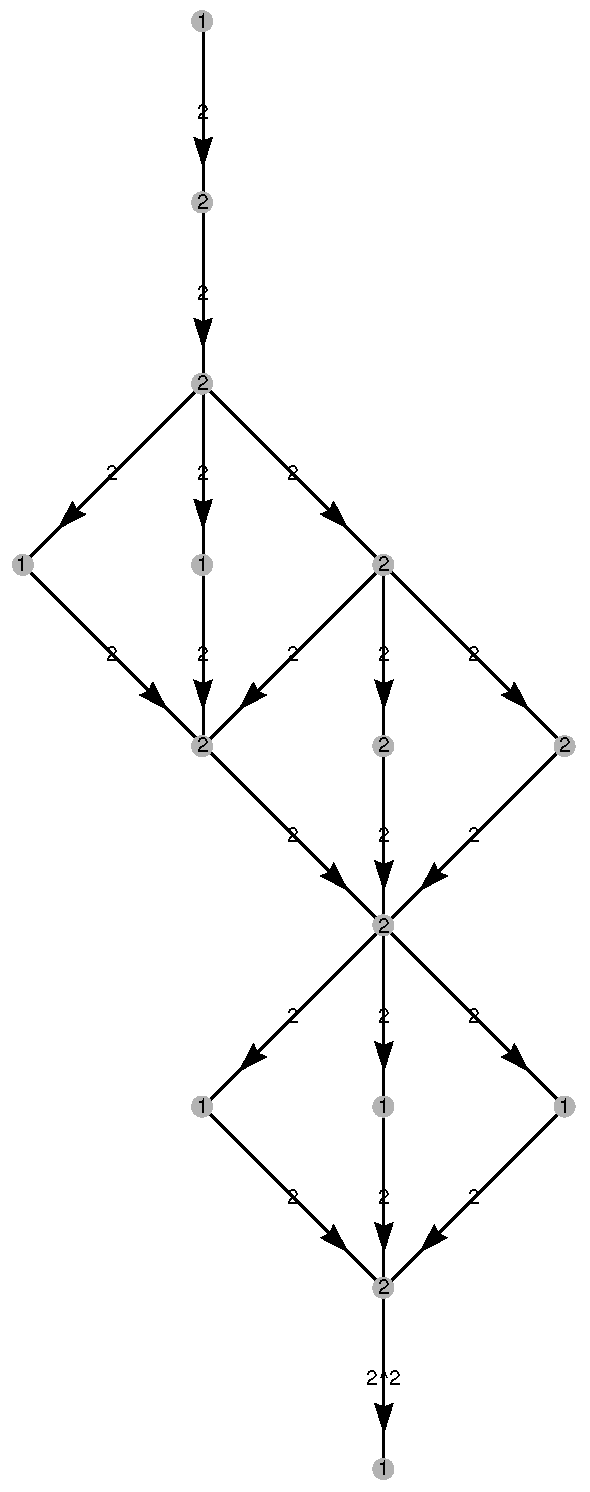
\includegraphics[width=0.65\textwidth]{graph-4}
%         \end{column}%
%         \begin{column}{0.6\textwidth}%
%             Weak equivalence classes of the monogenic order of $\Q[x]/(f)$ where $f=x^3+31x^2+43x+77$.\\
% 	    - vertices are orders, labeled by $\# \bWk$\\
% 	    - edges are inclusions, labeled by the index
%         \end{column}%
%     \end{columns}
% \end{figure}
% \end{frame}
% 
% \begin{frame}{Example 2}
% \vspace{-2 em}
% \begin{figure}
%     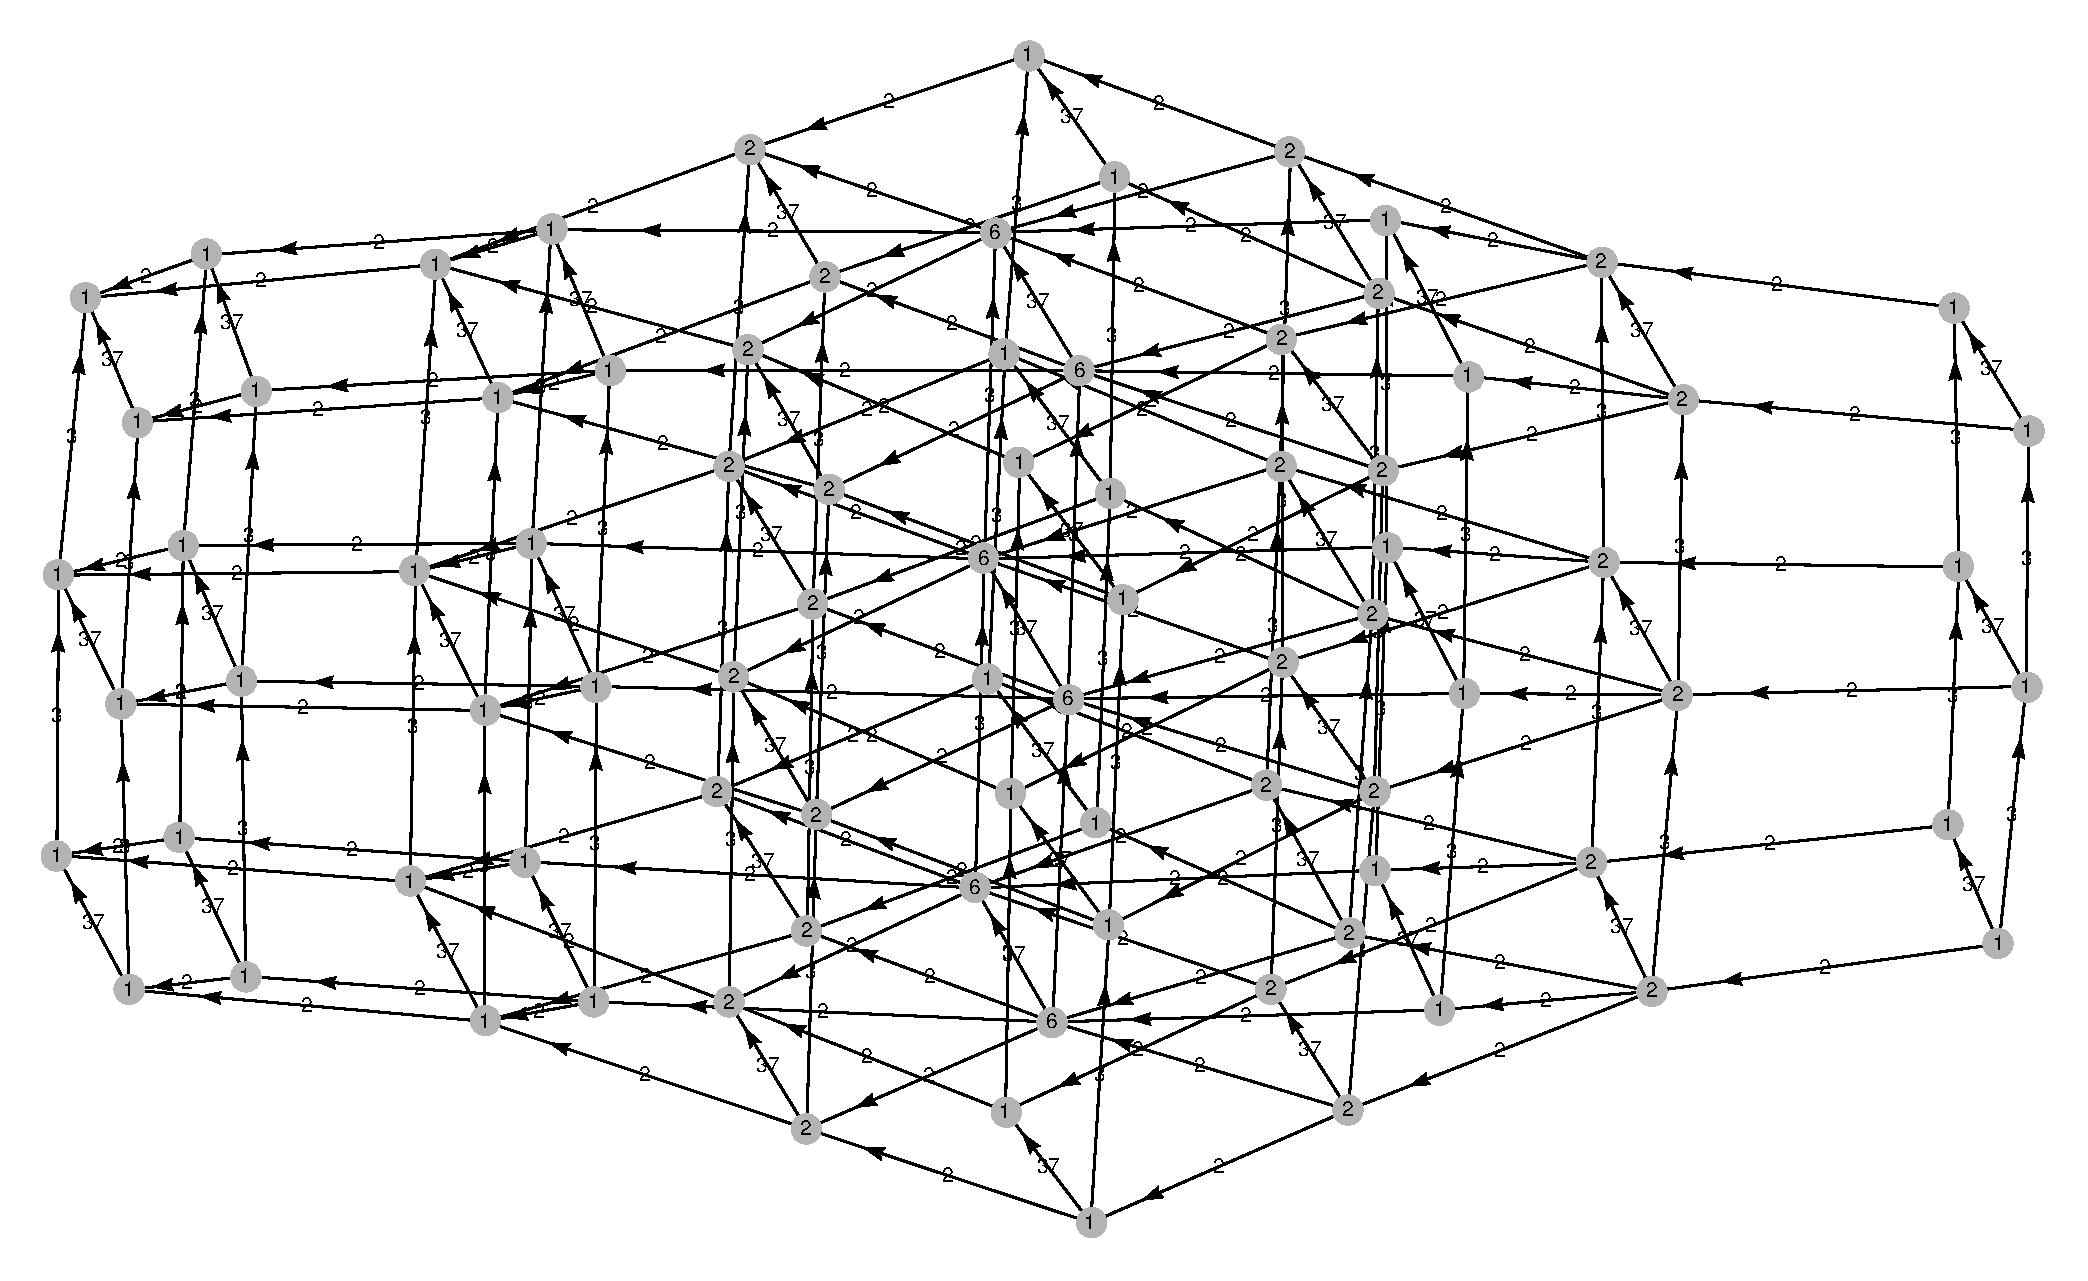
\includegraphics[width=1\textwidth]{graph-1}
% \end{figure}
% \vspace{-2 em} Weak equivalence classes of the monogenic order of $\Q[x]/(f)$ where
% \[ f=(x^2+4x+7)(x^3−9x^2−3x−1). \] 
% \end{frame}

\begin{frame}{ back to AV's: Dual variety/Polarization }
Howe described \textbf{dual} varieties and \textbf{polarizations} on Deligne modules.
\begin{theorem}[M.]
   If $A\leftrightarrow I$, then:
   \begin{itemize}
      \pause \item $A^\vee \leftrightarrow \overline{I}^t$.
      \pause \item a polarization $\mu$ of $A$ corresponds to a $\lambda\in K^\times$ such that\\
	    - $\lambda I \subseteq \overline{I}^t$ (isogeny);\\
	    - $\lambda$ is totally imaginary ($\overline \lambda = -\lambda$);\\
	    - $\lambda$ is $\Phi$-positive, where $\Phi$ is a specific CM-type of $K$.\\ 
      Also: $\deg \mu= [\overline{I}^t : \lambda I]$.
      \pause  \item if $(A,\mu) \leftrightarrow (I,\lambda)$ and $S=(I:I)$ then
     \vspace{-0.5em}
	      \[\set{\parbox[p]{7.5em}{non-isomorphic polarizations of $A$ of degree $=\deg\lambda$}} \longleftrightarrow \dfrac{\set{\text{totally positive }u\in S^\times }}{\set{v\overline{v}: v\in S^\times}}.\]
     \vspace{-1.5em}
	 \pause \item  $\Aut(A,\mu) = \set{\text{torsion units of $S$}}$.
\end{itemize}
\end{theorem}
\end{frame}

\begin{frame}{ Example}
\begin{itemize}
 \item Let $h(x)=x^8 - 5x^7 + 13x^6 - 25x^5 + 44x^4 - 75x^3 + 117x^2 - 135x + 81$.
 \item $\rightsquigarrow$ isogeny class of an simple ordinary abelian varieties over $\F_{3}$ of dimension $4$.
 \item Let $F$ be a root of $h(x)$ and put $R:=\Z[F,3/F]\subset \Q(F)$.
 \item $8$ over-orders of $R$: two of them are not Gorenstein.
 \item $\#\ICM(R) = 18 \rightsquigarrow 18$ isom.~classes of AV in the isogeny class.
 \item $5$ are not invertible in their multiplicator ring.
 \item $8$ classes admit principal polarizations.
 \item $10$ isomorphism classes of princ. polarized AV.
\end{itemize}
\end{frame}
\begin{frame}{Example}{}
Concretely:
{\scriptsize \begin{align*}
  \begin{split} 
  I_1 = & 2645633792595191 \Z \oplus (F + 836920075614551) \Z \oplus (F^2 + 1474295643839839)\Z \oplus\\
	& \oplus (F^3 + 1372829830503387)\Z \oplus (F^4 + 1072904687510)\Z \oplus\\
	& \oplus \frac{1}{3}(F^5 + F^4 + F^3 + 2F^2 + 2F + 6704806986143610)\Z \oplus\\
	& \oplus \frac{1}{9}(F^6 + F^5 + F^4 + 8F^3 + 2F^2 + 2991665243621169) \Z \oplus\\
	& \oplus \frac{1}{27}(F^7 + F^6 + F^5 + 17F^4 + 20F^3 + 9F^2 + 68015312518722201)\Z\\
  \end{split}
\intertext{principal polarizations:}
  \begin{split}
  x_{1,1} = \frac{1}{27}( & -121922F^7 + 588604F^6 - 1422437F^5 +\\
			  & +1464239F^4 + 1196576F^3 - 7570722F^2 + 15316479F - 12821193)\\ 
%   \end{split}\\
%   \begin{split}
  x_{1,2} = \frac{1}{27}( & 3015467F^7 - 17689816F^6 + 35965592F^5 -\\
			  & -64660346F^4 + 121230619F^3 - 191117052F^2 + 315021546F - 300025458)\\
  \end{split}\\
  & \End(I_1) =  R\\
  & \#\Aut(I_1,x_{1,1}) = \#\Aut(I_1,x_{1,2}) = 2
 \end{align*}}
\end{frame}


\begin{frame}{Example}
 
{\scriptsize \begin{align*}
  \begin{split} 
  I_7 = & 2\Z\oplus(F + 1)\Z\oplus(F^2 + 1)\Z\oplus(F^3 + 1)\Z\oplus(F^4 + 1)\Z\oplus\frac13(F^5 + F^4 + F^3 + 2F^2 + 2F + 3)\Z \oplus \\ 		      & \oplus\frac{1}{36}(F^6 + F^5 + 10F^4 + 26F^3 + 2F^2 + 27F + 45)\Z\oplus\\
	& \oplus \frac{1}{216}(F^7 + 4F^6 + 49F^5 + 200F^4 + 116F^3 + 105F^2 + 198F + 351)\Z\\
  \end{split}
\intertext{principal polarization:}\\[-7ex]
  \begin{split}
  x_{7,1} = \frac{1}{54}(20F^7 - 43F^6 + 155F^5 - 308F^4 + 580F^3 - 1116F^2 + 2205F - 1809)
  \end{split}\\
  \begin{split}
  \End(I_7) & = \Z \oplus  F\Z \oplus  F^2\Z \oplus  F^3\Z \oplus  F^4\Z \oplus
  \frac{1}{3}(F^5 + F^4 + F^3 + 2F^2 + 2F)\Z \oplus \\
	& \oplus \frac{1}{18}(F^6 + F^5 + 10F^4 + 8F^3 + 2F^2 + 9F + 9)\Z \oplus\\
	& \oplus \frac{1}{108}(F^7 + 4F^6 + 13F^5 + 56F^4 + 80F^3 + 33F^2 + 18F + 27)\Z\\
  \end{split}\\
  & \#\Aut(I_7,x_{7,1}) = 2
\end{align*}}             
$I_1$ is invertible in $R$, but $I_7$ is not invertible in $\End(I_7)$.
\end{frame}

\begin{frame}{ Final remarks }
\begin{itemize}
         \item Using Centeleghe-Stix '15 we can compute the isomorphism classes in $\cC_h$ over $\F_{\red{p}}$  where $h$ is \textbf{square-free} and \red{without real roots}.\\
\pause much larger subcategory!!!   
\pause   \item isogeny classes $\cC_{\red{h^d}}$ (with $h$ square-free) when $\Z[F,q/F]$ is Bass.
\pause   \item base field extensions and \green{twists} (ordinary case) (soon on arXiv).
\pause   \item \blue{period matrices} (ordinary case) of the canonical lift.
\pause 	 \item results of computations will appear on the LMFDB.
\end{itemize}
\end{frame}

\begin{frame}{ }
\begin{center}
{\Large Thank you!}
\end{center}
\end{frame}

\end{document}
